
%(BEGIN_QUESTION)
% Copyright 2016, Tony R. Kuphaldt, released under the Creative Commons Attribution License (v 1.0)
% This means you may do almost anything with this work of mine, so long as you give me proper credit

\noindent
{\bf Lab Exercise -- introduction}

\vskip 5pt

Your task is to build, document, and troubleshoot a liquid level measurement system consisting of a pneumatic $\Delta$P transmitter connected to a local ``receiver gauge'' pneumatic indicator as well as to a pressure transmitter to relay that same level measurement to a remotely-located electronic indicator.  Water held in a vertical tube is the suggested process variable to measure, but other liquid level variables are open for consideration, though.  Alternatives to the standard level-measurement lab are authorized by instructor permission only.

Part of this lab exercise is using a {\it liquid manometer} as a standard pressure-verification instrument.  Another part is the correct identification of common pipe and tube fittings.  A 3-valve or a 5-valve manifold must be attached to your transmitter for isolation and testing purposes.

The following table of objectives show what you and your team must complete within the scheduled time for this lab exercise.  Note how some of these objectives are individual, while others are for the team as a whole:

\underbar{Objective completion table:}

% No blank lines allowed between lines of an \halign structure!
% I use comments (%) instead, so that TeX doesn't choke.

$$\vbox{\offinterlineskip
\halign{\strut
\vrule \quad\hfil # \ \hfil & 
\vrule \quad\hfil # \ \hfil & 
\vrule \quad\hfil # \ \hfil & 
\vrule \quad\hfil # \ \hfil & 
\vrule \quad\hfil # \ \hfil & 
\vrule \quad\hfil # \ \hfil & 
\vrule \quad\hfil # \ \hfil \vrule \cr
\noalign{\hrule}
%
% First row
{\bf Performance objective} & {\bf Grading} & {\bf 1} & {\bf 2} & {\bf 3} & {\bf 4} & {\bf Team} \cr
%
\noalign{\hrule}
%
% Another row
Team meeting and prototype sketch (do {\it first!}) & mastery & -- & -- & -- & -- & \cr
%
\noalign{\hrule}
%
% Another row
Circuit design challenge & mastery & & & & & -- -- -- -- \cr
%
\noalign{\hrule}
%
% Another row
Final loop diagram and system inspection & mastery & & & & & -- -- -- -- \cr
%
\noalign{\hrule}
%
% Another row
Loop ranging ($\pm$ 1\% of span accuracy) & mastery & & & & & -- -- -- -- \cr
%
\noalign{\hrule}
%
% Another row
Manometer usage & mastery & & & & & -- -- -- -- \cr
%
\noalign{\hrule}
%
% Another row
Troubleshooting & mastery & & & & & -- -- -- -- \cr
%
\noalign{\hrule}
%
% Another row
Pipe and tube fitting identification & mastery & -- & -- & -- & -- & \cr
%
\noalign{\hrule}
%
% Another row
Lab question: Instrument connections & proportional &  &  &  &  & -- -- -- -- \cr
%
\noalign{\hrule}
%
% Another row
Lab question: Commissioning & proportional &  &  &  &  & -- -- -- -- \cr
%
\noalign{\hrule}
%
% Another row
Lab question: Mental math & proportional &  &  &  &  & -- -- -- -- \cr
%
\noalign{\hrule}
%
% Another row
Lab question: Diagnostics & proportional &  &  &  &  & -- -- -- -- \cr
%
\noalign{\hrule}
%
% Another row
Decommission and lab clean-up & mastery & -- & -- & -- & -- &  \cr
%
\noalign{\hrule}
} % End of \halign 
}$$ % End of \vbox

The only ``proportional'' scoring in this activity are the lab questions, which are answered by each student individually.  A listing of potential lab questions are shown at the end of this worksheet question.  The lab questions are intended to guide your labwork as much as they are intended to measure your comprehension, and as such the instructor may ask these questions of your team day by day, rather than all at once (on a single day).

\vskip 10pt

{\bf It is essential that your team plans ahead what to accomplish each day.  A short (10 minute) team meeting at the beginning of each lab session is a good way to do this, reviewing what's already been done, what's left to do, and what assessments you should be ready for.  There is a lot of work involved with building, documenting, and troubleshooting these working instrument systems!}

As you and your team work on this system, you will invariably encounter problems.  You should always attempt to solve these problems as a team before requesting instructor assistance.  If you still require instructor assistance, write your team's color on the lab whiteboard with a brief description of what you need help on.  The instructor will meet with each team in order they appear on the whiteboard to address these problems.





\vfil \eject

\noindent
{\bf Lab Exercise -- team meeting, prototype sketch, and instrument selection}

\vskip 5pt

An important first step in completing this lab exercise is to {\bf meet with your instructor} as a team to discuss safety concerns, team performance, and specific roles for team members.  If you would like to emphasize exposure to certain equipment (e.g. use a particular type of control system, certain power tools), techniques (e.g. fabrication), or tasks to improve your skill set, this is the time to make requests of your team so that your learning during this project will be maximized.

\vskip 10pt

An absolutely essential step in completing this lab exercise is to work together as a team to {\bf sketch a prototype diagram} showing what you intend to build.  This usually takes the form of a simple electrical schematic and/or loop diagram showing all electrical connections between components, as well as any tubing or piping for fluids.  This prototype sketch need not be exhaustive in detail, but it does need to show enough detail for the instructor to determine if all components will be correctly connected for their safe function.

For example, if you intend to connect field devices to a PLC (Programmable Logic Controller), your prototype sketch must show how those devices will connect to typical input/output terminals on the PLC, where electrical power will be supplied, etc.  Prototype sketches need not show all intermediary connections between components, such as terminal blocks in junction boxes between the field device and the controller.

You should practice good problem-solving techniques when creating your prototype sketch, such as consulting equipment manuals for information on component functions and marking directions of electric current, voltage polarities, and identifying electrical sources/loads.  Use this task as an opportunity to strengthen your analytical skills!  Remember that you will be challenged in this program to do all of this on your own (during ``capstone'' assessments), so do not make the mistake of relying on your teammates to figure this out for you -- instead, treat this as a problem {\it you} must solve and compare your results with those of your teammates.

Your team's prototype sketch is so important that the instructor will demand you provide this plan before any construction on your team's working system begins.  {\it Any team found constructing their system without a verified plan will be ordered to cease construction and not resume until a prototype plan has been drafted and approved!}  Similarly, you should not deviate from the prototype design without instructor approval, to ensure nothing will be done to harm equipment by way of incorrect connections.  Each member on the team should have ready access to this plan (ideally possessing their own copy of the plan) throughout the construction process.  Prototype design sketching is a skill and a habit you should cultivate in school and take with you in your new career.

\vskip 10pt

When selecting field instruments for this lab exercise, choose a {\it pneumatic $\Delta$P transmitter} -- ideally a Foxboro model 13A or model 15A -- and a valve ``manifold'' to isolate that transmitter from the hydrostatic pressure of the liquid column.  Refer to the ``Valve manifolds'' subsection of {\it Lessons In Industrial Instrumentation} for more detail on what these manifolds look like and how they are used.  You should choose a transmitter with a pressure range somewhere between 10 inches and 200 inches water column.  Avoid high-pressure transmitters ranged for hundreds or thousands of PSI.

Consult documentation from the manufacturer's website to identify how to properly wire, power, and calibrate the transmitter.  Your instructor will check to see you have located and are familiar with the equipment manual(s).

After locating a suitable instrument and its associated documentation, you should qualitatively test it prior to installing it in your system.  For a pneumatic pressure transmitter, this entails applying a low air pressure (blowing air using your mouth is usually adequate) to the ``high'' pressure port and measuring the transmitter's 3-15 PSI pneumatic output signal to see if it responds to the application of pressure.  If the transmitter fails to respond properly, tag it with a label explaining what it does (or what it fails to do).

For an indicator, you should use a {\it receiver gauge} designed to input a 3-15 PSI pressure signal, or a pneumatic controller (using the PV indicator).  Also connected to the transmitter's pneumatic output will be a standard electronic pressure transmitter ranged for 3-15 PSI, which will connect to an electronic controller or indicator as in the previous lab exercise (pressure measurement, INST240 sections 1 and 2).

\vskip 10pt

{\bf Planning a functioning system should take no more than an hour if the team is working efficiently, and will save you hours of frustration (and possible component destruction!).}







\vfil \eject

\noindent
{\bf Lab Exercise -- circuit design challenge}

\vskip 5pt

Connect a loop-powered ``smart'' differential pressure transmitter (4-20 mA output with HART communication ability) to a DC voltage source and a meter such that the meter will indicate a increasing signal when a certain stimulus is applied to the transmitter, setting the transmitter's pressure measurement range as specified by the instructor.  All electrical connections must be made using a terminal strip (no twisted wires, crimp splices, wire nuts, spring clips, or ``alligator'' clips permitted).  You are expected to supply your own tools and multimeter.

This exercise tests your ability to navigate a ``smart'' instrument's parameters using a communicator as well as properly interpret terminal connections on a field instrument for signal and power.

$$\includegraphics[width=15.5cm]{i00123x04.eps}$$

\vskip 10pt

The following components and materials will be available to you: assorted 2-wire 4-20 mA differential pressure {\bf transmitters} calibrated to ranges 0-30 PSI or less, equipped with Swagelok compression tube connectors at the ``high'' and ``low'' ports ; lengths of {\bf plastic tube} with ferrules pre-swaged ; {\bf terminal strips} ; lengths of {\bf hook-up wire} ; 250 $\Omega$ (or approximate) {\bf resistors} ; analog {\bf meters} ; {\bf battery clips} (holders); {\bf HART communicator}.

\vskip 10pt

\noindent
{\bf Transmitter range} (instructor chooses): \hskip 20pt LRV = \underbar{\hskip 50pt} \hskip 20pt URV = \underbar{\hskip 50pt}

\vskip 10pt

\noindent
{\bf Meter options} (instructor chooses): \hskip 20pt \underbar{\hskip 20pt} Voltmeter (1-5 VDC) \hskip 10pt {\it or} \hskip 10pt \underbar{\hskip 20pt} Ammeter (4-20 mA)

\vskip 10pt

\noindent
{\bf Signal increases with...} (instructor chooses): \hskip 20pt \underbar{\hskip 20pt} Positive pressure \hskip 10pt {\it or} \hskip 10pt \underbar{\hskip 20pt} Vacuum (suction)

\vskip 10pt

\vfil

Study reference: the ``Analog Electronic Instrumentation'' chapter of {\it Lessons In Industrial Instrumentation}, particularly the sections on loop-powered transmitters and current loop troubleshooting.  Also, the ``Basic Concept of HART'' subsection of the ``The HART Digital/Analog Hybrid Standard'' section of the ``Digital Data Acquisition and Networks'' chapter of the same book.






\vfil \eject

\noindent
{\bf Lab Exercise -- building the system}

\vskip 5pt

After getting your prototype sketch approved by the instructor, you are cleared to begin building your system.  Transmitters attach to 2-inch pipes using special brackets and U-bolts.  These brackets and U-bolts are located along with the transmitters in the instrument storage area.  Feel free to use 1/4 inch plastic tubing for all the pneumatic signal connections, and be sure not to exceed the rated supply pressure (as documented in the transmitter's manual).

Finally, your pressure-measurement system needs to have a loop number, so all instruments may be properly labeled.  This loop number needs to be unique, so that another team does not label their instruments and tubes the same as yours.  One way to make your loop number unique is to use the equivalent resistor color-code value for your team's color in the loop number.  For example, if you are the ``Red'' team, your loop number could be ``2''. 

Since this lab exercise follows the one focusing on pressure measurement, feel free to use the same electronic pressure transmitter from the previous lab exercise as the pneumatic-to-electronic signal converter in this lab exercise.  This will require re-ranging the pressure transmitter from whatever its previous range was to 3-15 PSI so it may properly receive the pneumatic level transmitter's pneumatic output signal.  In this new capacity, the electronic pressure transmitter will serve as a signal {\it converter} for the level signal (i.e. its ISA-standard tag will begin with ``LY'').  It is recommended that you use a different electronic indicator or indicating controller as the display unit on this lab exercise, to give yourself wider exposure to the controller/indicator options in our lab facility.  For example, if in the previous lab exercise your team used a panel-mount electronic indicating controller, consider using a PLC or a DCS as the electronic indicator in this lab exercise.

\vskip 10pt

{\bf Common mistakes:}

\begin{itemize}
\item{} Neglecting to consult the manufacturer's documentation for field instruments (e.g. how to connect pneumatic signal lines, how to calibrate them).
\item{} Mounting the field instrument(s) in awkward positions, making it difficult to reach tube connectors or to remove covers when installed.
\item{} Improper pipe/tube fitting installation (e.g. trying to thread tube fittings into pipe fittings and vice-versa).
\item{} Over-tightening tube fittings (remember, no more than 1-1/4 turns when assembling, and no more than ``snug'' when re-making the connection!).
\item{} Students working on portions of the system in isolation, not sharing with their teammates what they did and how.  It is important that the whole team learns all aspects of their system!
\end{itemize}

\vskip 10pt

\vfil \eject

It is relatively easy to construct a ``process vessel'' for measuring water level in, by using inexpensive PVC plastic piping and fittings:

$$\includegraphics[width=15.5cm]{i00123x02.eps}$$

Water is poured in the top, through the open tee fitting, and is drained through a valve at the bottom (preferably a 1/4 turn ball valve).

Even with an instrument valve manifold on the $\Delta$P transmitter, a shutoff valve is advisable between the process vessel connection and the transmitter to facilitate removal of the transmitter and manifold without having to drain the vessel.

\vskip 10pt

Note: The Foxboro model 13 and 15 pneumatic transmitters cannot handle large suppression values without the addition of a special ``suppression kit'' spring and screw adjustment to the transmitter mechanism.  When using the stock zero-adjust screw to account for suppression (the degree to which the transmitter's tube connection is below the LRV height on the vessel), be sure to position the transmitter so that the suppression is a small percentage of the measurement span. 

\vskip 10pt

{\bf Building a functioning system should take no more than one full lab session (3 hours) if all components are readily available and the team is working efficiently!}





\vfil \eject

\noindent
{\bf Lab Exercise -- documenting the system}

\vskip 5pt

Each student must sketch their own {\it loop diagram} for their team's system, following proper ISA conventions.  Sample loop diagrams are shown in the next question in this worksheet.  These loop diagrams must be {\it comprehensive} and {\it detailed}, showing every tube connection, every tube, range points, etc.  The principle to keep in mind here is to make the loop diagram so complete and unambiguous that anyone can follow it to see what connects to what, even someone unfamiliar with industrial instrumentation.  In industry, loops are often constructed by contract personnel with limited understanding of how the system is supposed to function.  The loop diagrams they follow must be so complete that they will be able to connect everything properly without necessarily understanding how it is supposed to work.

Every instrument and every signal tube and signal cable in your loop needs to be properly labeled with an ISA-standard tag number.  An easy way to do this is to wrap a short piece of masking tape around each tube (and placed on each instrument) then writing on that masking tape with a permanent marker.  Although no industry standard exists for labeling signal cables and tubes, a good recommendation is to label each tube with the tag number of the field instrument it goes to.  Thus, every length of tube in a pressure transmitter loop should be labeled ``PT-$x$'' (where ``$x$'' is the loop number), every flow control valve should be labeled ``FV-$x$'', etc.  Remember that the entire loop is defined by the process variable it measures: if the PV is {\it temperature} then the transmitter with be a {\it T}T, the control valve will be a {\it T}V, the controller with be a {\it T}C, etc.

Please note that this level-measurement system is part pneumatic and part electronic, and that your loop diagram must show {\it all} of these details.

When your entire team is finished drafting your individual loop diagrams, call the instructor to do an inspection of the loop.  Here, the instructor will have students take turns going through the entire loop, with the other students checking their diagrams for errors and omissions along the way.  During this time the instructor will also inspect the quality of the installation, identifying problems such as frayed wires, improperly crimped terminals, poor cable routing, missing labels, lack of wire duct covers, etc.  The team must correct all identified errors in order to receive credit for their system.  

After successfully passing the inspection, each team member needs to place their loop diagram in the diagram holder located in the middle of the lab behind the main control panel.  When it comes time to troubleshoot another team's system, this is where you will go to find a loop diagram for that system!

\vskip 10pt

{\bf Common mistakes:}

\begin{itemize}
\item{} Forgetting to label all signal tubes (see example loop diagrams).
\item{} Forgetting to label all field instruments with their own tag names (e.g. LT-83).
\item{} Forgetting to put your name on the loop diagram!
\item{} Basing your diagram off of a team-mate's diagram, rather than closely inspecting the system for yourself.
\item{} Not placing loop sheet instruments in the correct orientation (field instruments on the left, control room instruments on the right).
\end{itemize}

\vskip 10pt

{\bf Creating and inspecting accurate loop diagrams should take no more than one full lab session (3 hours) if the team is working efficiently!}





\vfil \eject

\noindent
{\bf Lab Exercise -- instrument calibration}

\vskip 5pt

Each student must calibrate their transmitter for a unique level measurement range, the LRV and URV points determined by the instructor (pieces of tape or zip-ties placed on the process vessel sightglass).  As in all cases where an instrument must be calibrated, you will need to check the instrument's response against one or more {\it standards}.  In this case, the ideal standard to use for setting the input (inches of water column pressure) to the transmitter is a {\it manometer}, and the ideal standard to use for measuring the transmitter's pneumatic output signal is a {\it precision test gauge} (either mechanical or electronic):

$$\includegraphics[width=15.5cm]{i00123x03.eps}$$

Read the ``Zero and Span Adjustments (Analog Instruments)'' section of {\it Lessons In Industrial Instrumentation} for more details on calibrating analog devices.  Note that the zero and span screw adjustments on pneumatic transmitters are interactive: adjusting the span will affect the zero, necessitating a lot of back-and-forth applications of LRV and URV, zero screw turning and span screw turning.

It is {\it strongly} recommended that you carefully measure the span of the level measurement range with a tape measure and calibrate your transmitter's span on the calibration bench as accurately as you can with a zero-based range (e.g. if the span is 35.1 inches, calibrate for a range of 0 to 35.1 inches), then field-set the transmitter's zero adjustment so that its output matches the actual level in the vessel (e.g. with an offset of 3.25 inches, that transmitter's range will now be 3.25 to 38.35 inches).  This procedure avoids the problem of trying to accurately measure the transmitter's zero offset (suppression) with a tape measure and wasting time on the bench adjusting the calibration pressure back and forth between two non-zero values as you repeat zero and span adjustments.  It also teaches the very practical concept of field-setting the zero of a transmitter.

{\bf Caution: the zero-adjust screw on the Foxboro pneumatic transmitter is quite delicate, and may easily be ruined if overtorqued.  Be especially careful not to turn the screw too far counter-clockwise and back it out of the nut, because it often cross-threads when subsequently turned the other way.  The simplest way to avoid problems here is to observe the zero screw and spring as you adjust it, making sure you do not over-compress the spring and/or back the screw out of the nut.}

\filbreak

Document the accuracy of your transmitter's calibration before and after adjustment in this table, at five different points throughout its sensing range using these two tables:

\vskip 10pt

{\bf As-Found calibration table}

% No blank lines allowed between lines of an \halign structure!
% I use comments (%) instead, so that TeX doesn't choke.

$$\vbox{\offinterlineskip
\halign{\strut
\vrule \quad\hfil # \ \hfil & 
\vrule \quad\hfil # \ \hfil & 
\vrule \quad\hfil # \ \hfil & 
\vrule \quad\hfil # \ \hfil \vrule \cr
\noalign{\hrule}
%
% First row
Applied pressure & Output signal (actual) & Output signal (ideal) & Error (\% of span) \cr
%
\noalign{\hrule}
%
% Another row
 &  &  & \cr
%
\noalign{\hrule}
%
% Another row
 &  &  & \cr
%
\noalign{\hrule}
%
% Another row
 &  &  & \cr
%
\noalign{\hrule}
%
% Another row
 &  &  & \cr
%
\noalign{\hrule}
%
% Another row
 &  &  & \cr
%
\noalign{\hrule}
} % End of \halign 
}$$ % End of \vbox

\vskip 10pt

{\bf As-Left calibration table}

% No blank lines allowed between lines of an \halign structure!
% I use comments (%) instead, so that TeX doesn't choke.

$$\vbox{\offinterlineskip
\halign{\strut
\vrule \quad\hfil # \ \hfil & 
\vrule \quad\hfil # \ \hfil & 
\vrule \quad\hfil # \ \hfil & 
\vrule \quad\hfil # \ \hfil \vrule \cr
\noalign{\hrule}
%
% First row
Applied pressure & Output signal (actual) & Output signal (ideal) & Error (\% of span) \cr
%
\noalign{\hrule}
%
% Another row
 &  &  & \cr
%
\noalign{\hrule}
%
% Another row
 &  &  & \cr
%
\noalign{\hrule}
%
% Another row
 &  &  & \cr
%
\noalign{\hrule}
%
% Another row
 &  &  & \cr
%
\noalign{\hrule}
%
% Another row
 &  &  & \cr
%
\noalign{\hrule}
} % End of \halign 
}$$ % End of \vbox

When finished calibrating your team's transmitter, be sure to place a calibration tag on it showing the range and the date it was calibrated.  A set of calibration tags are shown here which you may cut out and tape to the transmitter after completing your calibration:

$$\includegraphics[width=15.5cm]{i00123x01.eps}$$

The accuracy of your calibration will be checked by the instructor, filling and emptying your process vessel while checking the receiver gauge to make sure it reads 0\% at the LRV level and 100\% at the URV level.

\vskip 10pt

{\bf Common mistakes:}

\begin{itemize}
\item{} Applying excessive air pressure to a manometer, and blowing all the liquid out of it (when using a regulator as the calibration air pressure source)!
\item{} Applying excessive force to transmitter adjustments.  This is a delicate mechanism!  As such, it should {\it not} require forceful adjustment!!  If you have to {\it force} something, you're probably doing it wrong.
\item{} Improper supply air pressure to the transmitter (see the manual for supply air pressure specifications)
\item{} Failing to closely inspect pressure regulators before connecting them to an air source (e.g. connecting the air supply to the ``out'' port)
\item{} Improper pipe/tube fitting installation (e.g. trying to thread tube fittings into pipe fittings and vice-versa).
\item{} Poor tube connections, leading to air leaks which compromise the accuracy of the system.
\item{} Neglecting to place a calibration tag on the transmitter after calibrating it.
\item{} Forgetting to bleed all air out of the impulse line and transmitter body when installing the transmitter at the liquid process vessel (this will cause zero- and span-shift errors).
\end{itemize}






\vfil \eject

\noindent
{\bf Lab Exercise -- pipe and tube fitting identification}

\vskip 5pt

Part of this lab exercise is to properly identify the following types of pipe and instrument tube fittings from memory (without the aid of a pictorial reference).  Note that synonyms are separated by slash marks (e.g. ``street/run''):

\vskip 10pt

\noindent
{\bf Pipe fittings}

\begin{itemize}
\item{} Thread sizes: 1/8 inch NPT, 1/4 inch NPT, 3/8 inch NPT, and 1/2 inch NPT
\item{} Fitting type: tee (female, branch, and street/run)
\item{} Fitting type: elbow (female 45$^{o}$, female 90$^{o}$, and street)
\item{} Fitting type: cross
\item{} Fitting type: nipple  %INSTRUCTOR {\it (both male)}
\item{} Fitting type: coupling  %INSTRUCTOR {\it (same size, both female)}
\item{} Fitting type: reducing coupling  %INSTRUCTOR {\it (both female)}
\item{} Fitting type: reducing bushing  %INSTRUCTOR {\it (small female/large male)}
\item{} Fitting type: reducing adapter/expander  %INSTRUCTOR {\it (small male/large female)}
\item{} Fitting type: union
\item{} Fitting type: cap  %INSTRUCTOR {\it (female)}
\item{} Fitting type: plug  %INSTRUCTOR {\it (male)}
\item{} Fitting type: flange
\end{itemize}

\vskip 10pt

\noindent
{\bf Instrument tube fittings}

\begin{itemize}
\item{} Tube sizes: 1/8 inch, 1/4 inch, 3/8 inch, and 1/2 inch
\item{} Fitting components: nut and ferrule(s)
\item{} Fitting type: straight connector (male and female)
\item{} Fitting type: elbow connector (male and female)
\item{} Fitting type: union (straight and reducing)
\item{} Fitting type: tee (union, branch, run)
\item{} Fitting type: union elbow
\item{} Fitting type: union cross
\item{} Fitting type: bulkhead union
\item{} Fitting type: cap
\item{} Fitting type: plug
\end{itemize}

\vskip 10pt

A good way to prepare for this assessment is by working together as a team to identify random fittings in the pipe/tube drawers while referencing a manual such as the Parker and Swagelok fitting manuals contained in your Instrumentation reference.  The aspect of this assessment students find most challenging is identifying pipe thread sizes by sight.  Some black-iron pipe fittings have the fractional size (e.g. 1/2", 3/8", 1/2") cast into the fitting itself, which is probably your best guide to learning these thread sizes.

\vskip 10pt

{\bf In order to make this a practical as well as educational exercise, your team will identify different tube and pipe fittings while cleaning up and re-organizing the tube and pipe fitting collections in the lab.}  

\vskip 10pt






\vfil \eject

\noindent
{\bf Lab Exercise -- troubleshooting}

\vskip 5pt

The most challenging aspect of this lab exercise is {\it troubleshooting}, where you demonstrate your ability to logically isolate a problem in the system.  All troubleshooting is done on an individual basis (no team credit!), and must be done {\it on a system you did not help build}, so that you must rely on loop diagrams to find your way around the system instead of from your own memory of building it.

Each student is given 3 minutes to identify both the general location and nature of the fault, logically justifying all diagnostic steps taken.  All troubleshooting activities will take place under direct instructor supervision to ensure students are working independently and efficiently. 

Failure to correctly identify both the general location and nature of the fault within the allotted time, and/or failing to demonstrate rational diagnostic procedure to the supervising instructor will disqualify the effort, in which case the student must re-try with a different fault.  Multiple re-tries are permitted with no reduction in grade.

The instructor will review each troubleshooting effort after completion, highlighting good and bad points for the purpose of learning.  Troubleshooting is a skill born of practice and failure, so do not be disappointed in yourself if you must make multiple attempts to pass!  One of the important life-lessons embedded in this activity is how to deal with failure, because it {\it will} eventually happen to you on the job!  There is no dishonor in failing to properly diagnose a fault after doing your level best.  The only dishonor is in taking shortcuts or in giving up.

\vskip 10pt

{\bf Common mistakes:}

\begin{itemize}
\item{} Neglecting to observe pressure gauge indications.
\item{} Neglecting to use the three-valve manifold to perform diagnostic tests (e.g. block and equalize the transmitter to see whether or not its output pressure changes as input pressure is removed).
\item{} Neglecting to stimulate the flapper/nozzle mechanism as a diagnostic test, or stimulating it without observing the receiver gauge response.
\end{itemize}

\vskip 10pt

{\bf Remember that the purpose of the troubleshooting exercise is to foster and assess your ability to intelligently diagnose a complex system.  Finding the fault by luck, or by trial-and-error inspection, is not a successful demonstration of skill.  The only thing that counts as competence is your demonstrated ability to logically analyze and isolate the problem, correctly explaining all your steps!}

\vskip 10pt

{\bf Troubleshooting takes a lot of lab time, usually at least two 3-hour lab sessions for everyone in a full class to successfully pass.  Be sure your team budgets for this amount of time as you plan your work, and also be sure to take advantage of your freedom to observe others as they troubleshoot, to better learn this art.}



\vfil \eject

\noindent
{\bf Lab questions}

\vskip 5pt

\begin{itemize}
\item{} {\bf Instrument connections}
\item{} Determine correct tube connections between instruments to create a working 3-15 PSI pneumatic loop, based on diagrams of instruments with ports labeled
\end{itemize}

\filbreak

\begin{itemize}
\item{} {\bf Commissioning and Documentation}
\item{} Explain the operating principle of your pneumatic DP transmitter in as much detail as possible
\item{} Explain in detail how the {\it zero adjustment} on your transmitter functions; in other words, what is going on mechanically inside the transmitter as this adjustment is turned
\item{} Explain in detail how the {\it span adjustment} on your transmitter functions; in other words, what is going on mechanically inside the transmitter as this adjustment is turned
\item{} Identify the process ``bleed'' (``vent'') fittings on your pneumatic DP transmitter, and explain the significance of locating them in either a high or a low elevation on the flange of your transmitter
\item{} Identify and explain ``elevation'' and ``suppression'' as these terms apply to liquid level measurement using a $\Delta$P gauge or transmitter
\end{itemize}

\filbreak

\begin{itemize}
\item{} {\bf Mental math} (no calculator allowed!)
\item{} Calculate the correct pneumatic signal pressure (PSI) given a pressure transmitter calibration range and an applied pressure 
\item{} Calculate the pressure applied to a transmitter given a calibration range and the measured pneumatic signal pressure value
\item{} Calculate the percentage of span error for a transmitter given a calibration range and an As-Found calibration table 
\item{} Calculate the allowable level error for a transmitter given an allowable percentage of span error and a calibration range
\item{} Convert between different pressure units, without relying on the use of a reference for conversion factors (i.e. you must commit the major conversion factors to memory)
\end{itemize}

\filbreak

\begin{itemize}
\item{} {\bf Diagnostics}
\item{} Determine whether or not a given diagnostic test will provide useful information, given a set of symptoms exhibited by a failed system
\item{} Identify at least two plausible faults given the results of a diagnostic test and a set of symptoms exhibited by a failed system
\item{} Propose a diagnostic test for troubleshooting a failed system and then explain the meanings of two different test results
\end{itemize}



\vfil \eject

\noindent
{\bf Lab Exercise -- decommissioning and clean-up}

\vskip 5pt

The final step of this lab exercise is to decommission your team's entire system and re-stock certain components back to their proper storage locations, the purpose of which being to prepare the lab for the next lab exercise.  Remove your system documentation (e.g. loop diagram) from the common holding area, either discarding it or keeping it for your own records.  Also, remove instrument tag labels (e.g. FT-101) from instruments and from cables.  Perform general clean-up of your lab space, disposing of all trash, placing all tools back in their proper storage locations, sweeping up bits of wire off the floor and out of junction boxes, etc.

\vskip 10pt

\noindent
{\bf There are several steps you must follow in the decommissioning of the pneumatic DP transmitters:}

\begin{itemize}
\item{} Drain all water from transmitters before shelving them
\item{} Remove all mounting brackets from transmitters before shelving them
\item{} Remove all valve manifolds from transmitters before shelving them
\item{} Attach protective covers to all transmitters before shelving them
\item{} Cap all compression-style fittings so threads won't get damaged in storage
\end{itemize}


\vskip 10pt

\indent
{\bf Leave the following components in place, mounted on the racks:}

\begin{itemize}
\item{} Large control valves and positioners
\item{} I/P transducers
\item{} Large electric motors
\item{} Large variable-frequency drive (VFD) units
\item{} Cables inside conduit interconnecting junction boxes together
\item{} Pipe and tube fittings (do not unscrew pipe threads)
\item{} Supply air pressure regulators
\end{itemize}

\vskip 10pt

\indent
{\bf Return the following components to their proper storage locations:}

\begin{itemize}
\item{} Sensing elements (e.g. thermocouples, pH probes, etc.)
\item{} Process transmitters
\item{} ``Jumper'' cables used to connect terminal blocks within a single junction box
\item{} Plastic tubing and tube fittings (disconnect compression-style tube fittings)
\item{} Power cables and extension cords
\item{} Adjustment (loading station) air pressure regulators
\end{itemize}

\vskip 10pt

Finally, you shall return any control system components to their original (factory default) configurations.  This includes controller PID settings, function block programs, input signal ranges, etc.



\underbar{file i00123}
%(END_QUESTION)





%(BEGIN_ANSWER)


%(END_ANSWER)





%(BEGIN_NOTES)

\noindent
{\bf Loop diagrams / inspections:}

I strongly recommend checking off students' loop diagrams while you inspect their loop (checking for secure wiring, proper tubing, good conduit installation, etc.) with them.  Have all team members take you on a ``tour'' of their completed loop, with each team member explaining a different portion of the loop you select while using their own loop diagram as a guide.  While a student is explaining their section of the loop, you can check the other students' loop diagrams for accuracy.  This not only saves time by consolidating the tasks of loop inspection and loop diagram verification, but it also ensures students can actually relate their loop diagrams to the loop they have built and articulate that understanding to you.

\vskip 10pt

\goodbreak

\noindent
{\bf Troubleshooting fault ideas:}

\begin{itemize}
\goodbreak
\item{} Swap tube connections (construction fault)
\item{} Install pre-plugged orifice in transmitter
\item{} Turn supply air pressure well below 15 PSI
\item{} Miscalibrate transmitter and/or indicator/controller (inaccuracy fault)
\item{} Plug tube connections using portion of foam earplug stuffed into tube fitting (slow response fault)
\item{} Give students wrong loop diagram (documentation fault)
\item{} Close valve and leave safety tag hanging on it (operator/technician error)
\end{itemize}
















\vfil \eject

\noindent
{\bf Lab questions}

\vskip 20pt

\item{$(1)$} Sketch all the tube connections necessary to make this a working pneumatic pressure-measuring loop, where the DP transmitter senses a negative pressure (i.e. a vacuum) in the process vessel through the three-valve manifold and reports that measurement to the receiver gauge:

$$\includegraphics[width=15.5cm]{i00123x05.eps}$$

\vskip 20pt

\item{$(2)$} Explain in detail how the {\it zero adjustment} on your pneumatic transmitter functions; in other words, what is going on mechanically inside the transmitter as this adjustment is turned.  Please be detailed in your answer!

\vskip 20pt

\item{$(3)$} Identify the largest error in this As-Found calibration table for a pneumatic pressure transmitter with an input range of 0-200 inches water column and an output range of 3-15 PSI, and express that maximum error in terms of {\it percent of span}.  Be sure to specify whether the error is {\it positive} or {\it negative} (i.e. the instrument registers more than it should or less than it should):

% No blank lines allowed between lines of an \halign structure!
% I use comments (%) instead, so that TeX doesn't choke.

$$\vbox{\offinterlineskip
\halign{\strut
\vrule \quad\hfil # \ \hfil & 
\vrule \quad\hfil # \ \hfil \vrule \cr
\noalign{\hrule}
%
% First row
{\bf Input} & {\bf Output} \cr
%
\noalign{\hrule}
%
% Another row
0 inches W.C. & 3.05 PSI \cr
%
\noalign{\hrule}
%
% Another row
75 inches W.C. & 6.02 PSI \cr
%
\noalign{\hrule}
%
% Another row
150 inches W.C. & 9.00 PSI \cr
%
\noalign{\hrule}
%
% Another row
225 inches W.C. & 11.92 PSI \cr
%
\noalign{\hrule}
%
% Another row
300 inches W.C. & 14.96 PSI \cr
%
\noalign{\hrule}
} % End of \halign 
}$$ % End of \vbox

\vskip 20pt

\item{$(4)$} Suppose a pneumatic level transmitter senses liquid level by that liquid's hydrostatic pressure, and reports the level measurement to a 3-15 PSI ``receiver gauge'' located in the control room.  One day the operator notices the receiver gauge registers well over 100\% level but knows the vessel is only about 40\% full by visual inspection.  A technician decides to test the transmitter by pulling its flapper (baffle) away from its nozzle while asking the operator to view the receiver gauge's indication.  Is this a useful diagnostic test?  Explain why or why not.


















\vfil \eject

\noindent
{\bf Lab questions}

\vskip 20pt

\item{$(1)$} Sketch all the tube connections necessary to make this a working pneumatic pressure-measuring loop, where the DP transmitter senses a positive pressure in the process vessel through the three-valve manifold and reports that measurement to the receiver gauge:

$$\includegraphics[width=15.5cm]{i00123x05.eps}$$

\vskip 20pt

\item{$(2)$} Explain in detail how the {\it span adjustment} on your pneumatic transmitter functions; in other words, what is going on mechanically inside the transmitter as this adjustment is turned.  Please be detailed in your answer!

\vskip 20pt

\item{$(3)$} Identify the largest error in this As-Found calibration table for a pneumatic pressure transmitter with an input range of 0-200 inches water column and an output range of 3-15 PSI, and express that maximum error in terms of {\it percent of span}.  Be sure to specify whether the error is {\it positive} or {\it negative} (i.e. the instrument registers more than it should or less than it should):

% No blank lines allowed between lines of an \halign structure!
% I use comments (%) instead, so that TeX doesn't choke.

$$\vbox{\offinterlineskip
\halign{\strut
\vrule \quad\hfil # \ \hfil & 
\vrule \quad\hfil # \ \hfil \vrule \cr
\noalign{\hrule}
%
% First row
{\bf Input} & {\bf Output} \cr
%
\noalign{\hrule}
%
% Another row
0 inches W.C. & 3.01 PSI \cr
%
\noalign{\hrule}
%
% Another row
50 inches W.C. & 5.98 PSI \cr
%
\noalign{\hrule}
%
% Another row
100 inches W.C. & 8.99 PSI \cr
%
\noalign{\hrule}
%
% Another row
150 inches W.C. & 12.05 PSI \cr
%
\noalign{\hrule}
%
% Another row
200 inches W.C. & 15.10 PSI \cr
%
\noalign{\hrule}
} % End of \halign 
}$$ % End of \vbox

\vskip 20pt

\item{$(4)$} Suppose a pneumatic level transmitter senses liquid level by that liquid's hydrostatic pressure, and reports the level measurement to a 3-15 PSI ``receiver gauge'' located in the control room.  One day the operator notices the receiver gauge registers well below 0\% level but knows the vessel is over half-full by visual inspection.  A technician decides to test the transmitter by pulling its flapper (baffle) away from its nozzle while asking the operator to view the receiver gauge's indication.  Is this a useful diagnostic test?  Explain why or why not.



%INDEX% Lab exercise, liquid level measurement loop
%INDEX% Lab exercise, manometer usage
%INDEX% Lab exercise, pneumatic DP transmitter

%(END_NOTES)




